\documentclass[a4paper,12pt,twoside]{article}
\usepackage[papersize={8.5in,11in},left=2.64cm,right=2.64cm,top=2.64cm,bottom=2.64cm]{geometry}

\usepackage{natbib}
\usepackage{lineno}
\usepackage{soul}
\usepackage{url}
\usepackage[colorlinks = true,
            linkcolor = blue,
            urlcolor  = blue,
            citecolor = blue,
            anchorcolor = blue]{hyperref}
            
\linenumbers
\usepackage[printfigures]{figcaps}

\setlength{\marginparwidth}{2cm}
\usepackage[colorinlistoftodos,prependcaption,textsize=tiny]{todonotes}
\usepackage{authblk}
\usepackage{setspace}
\doublespacing

\usepackage{inputenc}

\def\keywords{\vskip4pt\vskip0sp\subsection*{Key words:}
\begin{itemize}}
\def\endkeywords{\end{itemize}}

\def\keypoints{\vskip4pt\vskip0sp\subsection*{Key points:}
\begin{itemize}}
\def\endkeypoints{\end{itemize}}



%opening
\title{The imbricated foreshock and aftershock activities of the Balsorano (Italy) M$_w$ 4.4 normal fault earthquake and implications for earthquake initiation}

\author{H. S. S\'anchez-Reyes$^1$, D. Essing$^1$, E. Beauc\'e$^2$, P. Poli$^1$}

\affil[1]{Institute of Earth Sciences, University Grenoble Alpes, Grenoble \emph{38100}, France}
\affil[2]{Department of Earth, Atmospheric, and Planetary Sciences, Massachusetts Institute of Technology, Cambridge, MA, United States}
\affil[*]{Corresponding author: hugo.sanchez-reyes@univ-grenoble-alpes.fr}

\date{}                     %% if you don't need date to appear
\setcounter{Maxaffil}{0}
\renewcommand\Affilfont{\itshape\small}



\begin{document}


\maketitle

\pagebreak

\begin{keywords} 
\item earthquake initiation process
\item earthquake sequence
\item spatio-temporal evolution 
\end{keywords} 

\begin{keypoints}
\item The analysis of the 2019 Balsorano earthquake sequence reveals that imbricated complex processes occur before and after the main earthquake
\item Clear differences between foreshocks and aftershocks are highlighted by the distinct spatio-temporal patterns unraveled by our analysis
\item These results demonstrate that simple earthquake preparation models are not suitable enough to correctly mimic the observed complex reality
\end{keypoints}


\pagebreak


\begin{abstract}

Foreshocks in the form of microseismicity are among the most powerful tools to study the physical processes that occur before main earthquakes. However, their detection and precise characterization is still sparse, especially for relatively small earthquakes (M$_w<5$). We present here a detailed foreshock analysis for the November 7, 2019, Balsorano (Italy) normal fault earthquake (M$_w$ 4.4). To improve the detection of the microseismicity before and after the mainshock, we use six three-component broadband receivers at distances of less than 75 km from the targeted seismicity, through template matching. To improve the understanding of the physical mechanism(s) behind the earthquake initiation process, as well as other accompanying phenomena, we also detail the spatio-temporal evolution of the sequence associated to this medium-sized earthquake, using waveform clustering and hypocenter relocation. Clear differences between foreshocks and aftershocks are revealed by this analysis. Moreover, five distinct spatio-temporal patterns associated to the different seismic activities are revealed. The observed spatio-temporal behavior shown by the foreshocks highlights a complex initiation process, which apparently starts on an adjacent unmapped antithetic fault. Finally, the aftershock activity comprises four different clusters with distinct spatio-temporal patterns, which suggests that each cluster in this sequence has a distinct triggering mechanism.

\end{abstract}


\section*{Introduction}

The detection of signals that can inform us about an incoming earthquake is fundamental to build physical models that mimic the processes behind the triggering of earthquakes. Over the last 25 years, numerous studies have reported a wide range of observations that appear to be connected with the physics that precedes large seismic events \citep[\emph{e.g.}][]{Rikitake_1975_EP, Jones_1979_SCF, Molchanov_1998_PES, Eftaxias_2000_DEE, Virk_2001_HRP, Singh_2010_PSU, DeSantins_2019_PWS, Jones_1985_FTE, Abercrombie_1996_OPF, Felzer_2004_COA, Dodge_1996_DOC, Ellsworth_2018_NIE, Yoon_2019_FMN, Reasenberg_1999_FOB, ruiz2017nucleation, ruiz2014intense}. Among these, the more significant ones have been based on seismological characterization of foreshock sequences and their relationships with mainshocks \citep[\emph{e.g.}][]{Jones_1985_FTE, Abercrombie_1996_OPF, Reasenberg_1999_FOB, Felzer_2004_COA, Dodge_1996_DOC, Ellsworth_2018_NIE, Yoon_2019_FMN, ruiz2017nucleation}. Foreshocks are thus one of the most useful tools to understand the physics of earthquake initiation in real faults \citep{Brune_1979_IET, Abercrombie_1996_OPF, Malin_2018_MPE}. Therefore, it is important to improve foreshock observations and characterization, even for frequent medium-sized events (\emph{i.e.} M$_w <$ 6), as these might share similar physical processes with larger events. These improved observations shed new light on the physical processes that occur during the triggering of earthquakes and will drive future research that focuses on theoretical and numerical models to better characterize earthquake occurrence in real and complex faults. 

Earthquake initiation \citep[\emph{e.g.}][]{Kato_2012_PSS, Schurr_2014_GUP, Tramutoli_2015_VCR} and earthquake nucleation/triggering \citep[\emph{e.g.}][]{Dieterich_1992_ENF, Ellsworth_1995_SEE, Rubin_2005_ENR} are two different, and perhaps overlapping, phases of the seismic cycle. While the first is understood to occur over the longer term preceding a large event (\emph{i.e.}, days or months, to years), the second occurs some minutes to seconds before the main event. Both phases, however, can be explained under the Dieterich model (\citeyear{Dieterich_1994_CLR}), which relates the seismicity rate to the stressing history through a rate-and-state constitutive law. For earthquake initiation in particular for real faults, two main hypotheses are currently used to explain this process. Some authors argue that a mainshock is a consequence of a cascade process, with stress transfer in-between events, which eventually trigger the large event \citep[\emph{e.g.},][]{Dodge_1996_DOC, Ellsworth_2018_NIE, Yoon_2019_FMN}. Alternatively, the initiation of an earthquake can be understood as an aseismic process that weakens the pre-existing asperities, until a larger rupture is promoted \citep{Dodge_1996_DOC, Bouchon_2011_ENI, Tape_2018_ENF}. In the latter case, foreshocks result from the activation of brittle asperities by the surrounding slip processes. However, intermediate models that involve both triggering and aseismic slip are likely for complex faults \citep[\emph{e.g.}][]{mclaskey2019earthquake}. This complexity might result from fault heterogeneity (\emph{e.g.}, variable stress, frictional properties) and promote imbricated sequences of foreshocks and aseismic slip \citep[\emph{e.g.},][]{dublanchet2018dynamics}.

The monitoring of foreshocks is today routine in laboratory experiments \citep[][and references therein]{Zang_1998_SAA, Goebel_2012_IFH, Renard_2019_VSP}, while  studies that focus on large earthquakes remain relatively sparse (\emph{i.e.}, M$_w>$6) \citep[\emph{e.g.},][]{Mogi_1963_SDA, Abercrombie_1996_OPF, Kato_2012_PSS, Chen_2013_CFS, Bouchon_2013_LPP, Ruiz_2014_IFS, ruiz2014intense}. However, the recent improvements to seismological monitoring systems around active faults have now provided detailed analysis of foreshocks that precede the more frequent small-magnitude earthquakes (M$_w <$ 6) \citep[\emph{e.g.},][]{Savage_2017_PPS, Mcmahon_2017_STE, Malin_2018_MPE}. One intriguing feature that has emerged from these last more recent studies is the increased complexity (\emph{i.e.}, fault interactions, volumetric processes) that have been revealed through the availability of better data (\emph{e.g.}, near-fault receivers) and more advanced detection methods (\emph{e.g.}, template matching) to study foreshocks. This complexity might challenge the actual laboratory scale and theoretical models, which treat earthquake initiation as simple physical processes that occur in smooth fault planes \citep{Dieterich_1992_ENF, Marone_1998_ELR, Rubin_2005_ENR, Liu_2005_AST}. The necessity for high-resolution characterization of foreshocks based on good data and advanced data processing techniques was also suggested by a meta-analysis carried out by \cite{Mignan_2014_DPV}, which indicated resolution-dependent bias for earthquake initiation models that were resolved using seismological data. 

To shed new light on the physical processes that occur before relatively small earthquakes, we study here the medium-sized (M$_w$ 4.4) Balsorano normal fault earthquake and its foreshock-aftershock sequence (Fig. 1). The Italian National Institute of Geophysics and Volcanology (\emph{Istituto Nazionale di Geofisica e Vulcanologia}; INGV; \href{http://terremoti.ingv.it/it/event/23414191}{\color{blue}online catalog}) reported that the main event of this sequence occurred on November 7, 2019 (17:35:21.18 UTC), approximately 4 km southeast of Balsorano city in central Italy (Fig. 1). The hypocenter of this main event was located relatively deep in the crust ($\sim$ 15 km), close to the transition zone between the upper and lower crust (10-20 km in depth), where the brittle locked fault transitions into the ductile regime zone \citep{Doglion_2011_RBD}. Below this depth, the lower crust is relatively seismically silent \citep{Doglion_2011_RBD}. According to a geological study of the location of the main event and its focal mechanism (Supplementary Material Table S1), this event ruptured the Liri fault \citep{Roberts_2004_STV}, which is one of the major active normal faults mapped in this region. This structure accommodates the  low extension rate observed in this region (\emph{i.e.}, a few millimeters per year) \citep{Hunstad_1999_UBR, Westaway_1992_SMS, Dagostino_2001a_ACE, Roberts_2004_STV}.

\begin{center}
   [Figure 1]
\end{center}


\begin{figure}
    \centering
     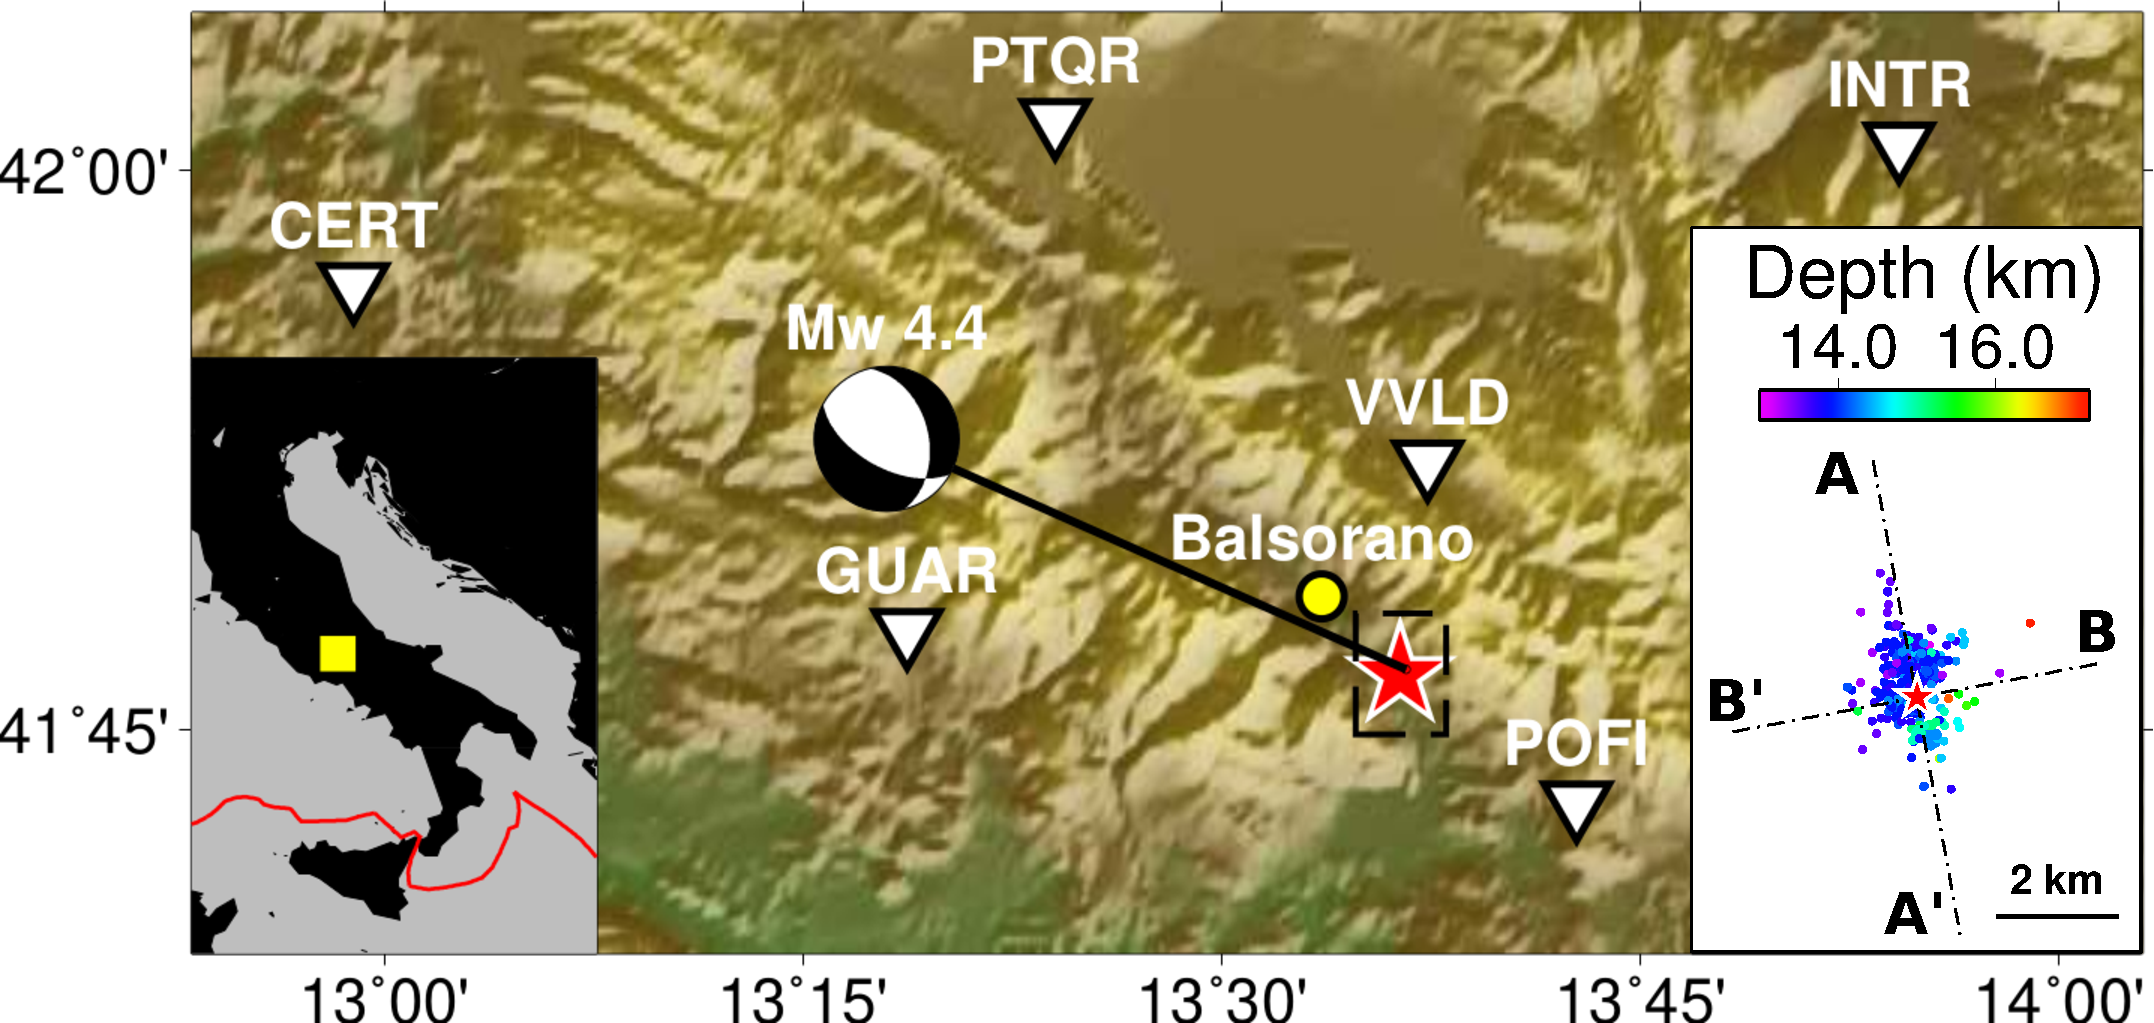
\includegraphics[width=1\linewidth]{map_balsorano.pdf}
    \caption{Regional map of the study area. The yellow square inside the small map inset on the left corresponds to the central region of Italy represented in the larger topographic map. The small map inset on the right represents magnification of the black dashed area around the epicentral location (red star). The color code used in the map view on the right represents the estimated depth of the foreshock and aftershock activity (estimated in this study: 714 events). The yellow circle represents Balsorano city, and the white triangles represent the stations used in this study. The dashed lines in the right inset map represent the directions A-A' (along strike) and B-B' (normal to the strike) illustrated in the cross sections of Figure 5.}
\end{figure}    \label{fig:general_map}

In addition to the mainshock of November 7, 2019, 135 events occurred close to the epicenter of the main event from October 22 to November 15, 2019 (which included 25 foreshocks). Starting from these cataloged events, we study here the 'anatomy' of the foreshocks and aftershocks, and their relationships with the main event. With this aim, continuous data from six three-component stations at less than 75 km from the mainshock epicenter are used (Fig. 1; Supplementary Materials Table S2). The continuous waveforms recorded are analyzed using template matching techniques \citep{Gibbons_2006_DLM, Shelly_2007_CET} to detect smaller events and thus to expand upon the available seismic catalog. The detected events are then relocated using the double-difference method \citep{Waldhauser_2001_HDD}, to reveal the geometry of the main fault and to obtain new insights into the fault-slip behavior(s) before and after the main seismic event. Furthermore, through waveform clustering, we isolate families of earthquakes that are representative of different physical processes that occur in the pre- and post-mainshock period. This combination of detection, relocation, and waveform clustering reveals an imbricated seismic sequence where several faults were activated, and with clear differences in the spatio-temporal properties of the foreshocks and aftershocks.

\section*{Methods} 
\label{sec:methods}

{\bf Template matching:} The analysis starts by extending the INGV seismic catalog using the template matching approach \citep{Gibbons_2006_DLM}. From the 135 events reported by the INGV online catalog \href{http://terremoti.ingv.it/en}, where 25 events are identified as foreshocks, we retain only the events with available P-wave and S-wave picks for all of the six stations used. We then extract 4 s of signal, starting 1 s before the phase arrival time from the band-pass filtered data (5-20 Hz). Using the pre-picked signals, we estimate the signal-to-noise ratio and retain as templates only those events with a signal-to-noise ratio $>$3 at all of the stations. With this data selection, 23 events are obtained (including three foreshocks) that are the templates used for scanning the continuous data (Supplementary Materials Table S4). We use three-component data with P waves extracted from the vertical component, and S waves extracted from the East and North components.

In all, 28 days of continuous data are processed, from October 22 (\emph{i.e.}, 16 days before the mainshock) to November 15, 2019, using the fast matched filter algorithm from \cite{Beauce_2017_FMF}. The detection thresholds are set to 12 times the daily median absolute deviation of the summed correlation coefficients over the array of stations. Finally, consecutive detections with differential times of $<$3 s are removed (\emph{i.e.}, the time difference between two estimated origin times).

The final catalog contains 714 events (166 foreshocks, 547 aftershocks), which represents $\sim$ 6-fold the number of events in the initial catalog. To estimate the magnitudes of the newly detected events, we use the average root mean square in the time window containing the S waves over all of the stations and components. Least-square fitting is then used to obtain a linear model that relates the logarithmic of the root mean square of the 23 templates and their local magnitudes from the INGV catalog. This model is then used to estimate the magnitude of the newly detected events. A summary of the event occurrences in time together with their magnitudes is shown in Figure 2.

\begin{center}
   [Figure 2]
\end{center}

\begin{figure}
    \centering
     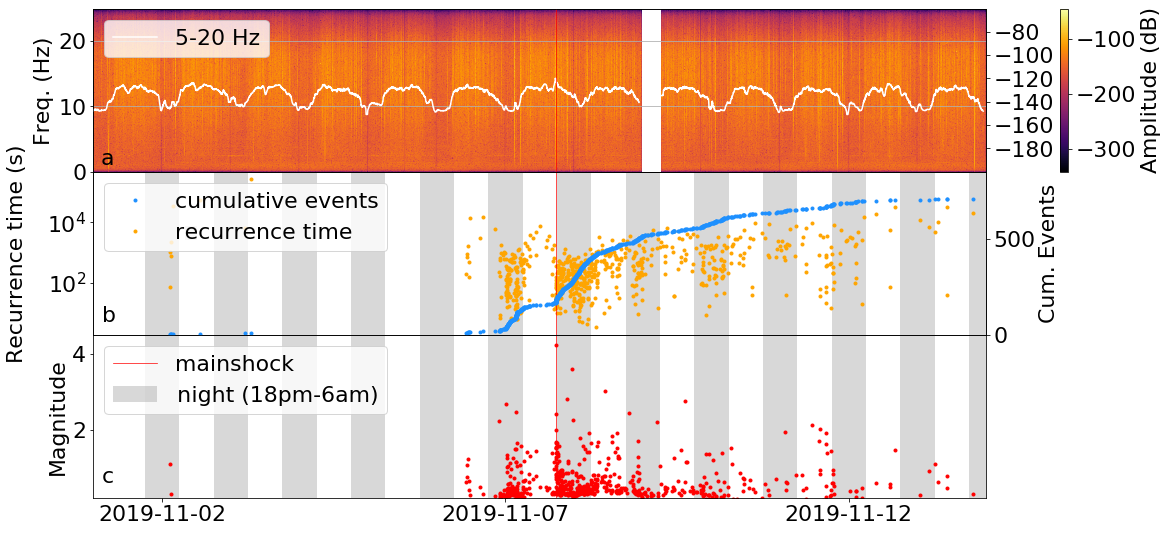
\includegraphics[width=1\linewidth]{spec_rec_mag.png}    \caption{(a) Spectrogram on VVLD.HHZ. The white line is the median of the energy in the frequency band between 5 Hz and 20 Hz calculated within a 1-h sliding window. (b) Blue, cumulative events for the same time period of the experiment; orange, recurrence time for the newly detected events. (c) Estimated magnitudes for the newly detected events. A gap in the continuous data at this receiver location is seen for the night of November 8 to 9, 2019.}
\end{figure}    \label{fig:spectrum}


{\bf Waveform-based clustering:} Clustering is widely used in seismology to recognize patterns in spatio-temporal events, which include the identification of foreshock-aftershock sequences and stress evolution in time \citep[\emph{e.g.},][]{Kagan_1991_LTE, wehling_2013_IDT, Cesca_2014_SMC, Ellsworth_2018_NIE}. Here, we apply waveform similarity analysis \citep{Cattaneo_1999_WSA} to define groups of events that share similar locations and/or a common rupture mechanism \citep{Kagan_1991_LTE, wehling_2013_IDT, Cesca_2014_SMC, Ellsworth_2018_NIE, Cattaneo_1999_WSA}. For this, the full normalized waveforms are used, with a 4.5-s time window (starting 0.5 s before the P-wave arrival) that contains both the P phase and the S phase. 

The waveforms of the 714 detected events recorded at the closest station to the epicenter (Fig. 1, VVLD) are then correlated with each other. The correlation matrix obtained (Fig. 3a) is used to estimate the distance (dissimilarity) metric to perform hierarchical clustering. The Ward minimum variance method is used \citep{Ward_1963_HGO} with  a distance threshold of 5.5 defined (Supplementary Materials Fig. S1: the largest separation observed from the dendrogram). This waveform similarity analysis highlights five different clusters, as shown in Figure 3b, c. As both the P waves and S waves are used for clustering, the resulting family members should share similarities in position and rupture mechanism \citep{Kagan_1991_LTE, wehling_2013_IDT, Cesca_2014_SMC, Ellsworth_2018_NIE, Cattaneo_1999_WSA}.

{\bf Relocation:} We finally estimate the relative location between the detected events using the double-difference algorithm (HypoDD software; \cite{Waldhauser_2001_HDD}). The differential times of the P phases and S phases between events from the cross-correlation are estimated, with the retention of only the delays that are associated to correlation coefficients $>$0.6. We further limit the delays to 0.2 s. After discarding the event pairs that relate less than 3 P-wave and 3 S-wave highly correlated differential times (correlation coefficient, $\geq$ 0.6), the final number of 29859 pairs are kept and used in the relocation process. 

For each newly detected event, we assume its initial location as the coordinates of the template that reports the highest correlation coefficient related to that event. In addition, we assume the estimated P-wave and S-wave picks obtained from our template matching analysis as the initial catalog information for the relocation. A velocity model for this region proposed by \cite{Bagh_2007_BSC} is used in the relocation process (Supplementary Materials Table S3). Following previous studies \citep{Shelly_2019_IFC}, the inversion is performed with stronger weights to the initial information related to the P-wave and S-wave picks from the catalog (\emph{i.e.}, from the template matching analysis), while the differential times from the waveform correlations control the final iterations. In the end, 689 of the 714 newly detected events are successfully relocated. The temporal and geometric patterns observed in this earthquake sequence are illustrated in Figures 4 and 5, and are further described in the following section.

\begin{center}
   [Figure 3]
\end{center}

\begin{figure}
    \centering
     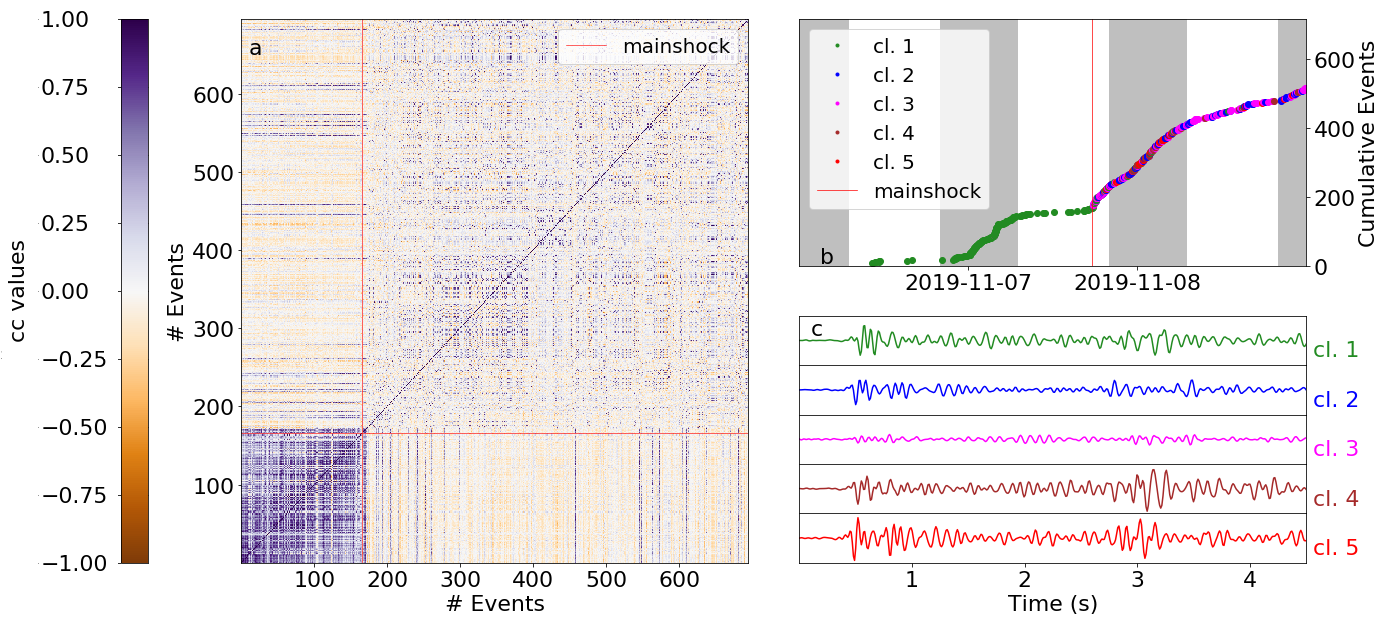
\includegraphics[width=1\linewidth]{wigg_cc_mat_cluster.png}    \caption{Illustration of the waveform-based hierarchical clustering output. (a) Pairwise correlation coefficients between the waveforms for the vertical component of station VVLD (Fig. 1) of the 714 detected events. This matrix is used to perform the hierarchical clustering. (b) Cumulative events combined with the results from the hierarchical clustering, according to the color code in the legend. (c) Characteristic normalized waveforms (vertical component) of the five different clusters revealed in the earthquake sequence. These traces are obtained after stacking all of the individually normalized waveforms belonging to each cluster.}
\end{figure}    \label{fig:declustering}


\section*{Results and discussion}
\label{sec:results}

The time evolution of the detected events is shown in Figure 2. Of the 714 events, 166 are foreshocks (23\%). Together with the temporal evolution, Figure 2a shows the spectrogram and the average spectral energy in a frequency band from 5 Hz to 20 Hz. The oscillation of this energy suggests variable noise levels in the study area, with lower noise during the night (Figure 2, shaded areas, for periods from 18:00 to 06:00). This noise variation is related to anthropogenic activity \citep{Poli_2020}, and it is also observed for the other five receivers. This noise evolution will probably affect our detection performance. For example, it is not clear if the reduced number of events observed prior to the mainshock is real or is a consequence of the higher noise level (Fig. 2b). We thus avoid discussing any issue related to pre-seismic quiescience here. However, with the geometric and clustering information derived above, we can still characterize some of the properties of the newly detected foreshocks and aftershocks, and gain insight into the physical processes that occur at the different stages of the sequence.

The results from the combination of waveform clustering and relocation strategies are summarized in Figures 4 and 5. For each cluster, the coefficient of variation (COV) is also estimated from the recurrence time of the events \citep{Kagan_1991_LTE, Schoenball_2017_SAS}. The COV indicates the level of the temporal clustering within each group (\textit{i.e.}, how much the occurrence of future earthquakes depends on the occurrence of the past earthquakes): with COV=1 for random seismicity, and COV$>$1 for strong temporal clustering. The larger the COV, the more the earthquakes are interacting. Thus, it is important to note that events that happen together with a high COV mean that there is an intrinsically related interaction between them.

The temporal and spatial densities of the different clusters identified in this sequence are illustrated in Figure 4, where cluster 1 (green solid lines and dots) is mainly composed of foreshocks (161 of 209 events occurred before the mainshock). The events that form this family show the highest waveform similarity (Fig. 3a). In agreement with this waveform property, cluster 1 has high spatial density, with approximately 90\% of its activity (193 of the 208 events) located within 0.5 km of the mainshock hypocenter (Figs. 4a and 5a). Cluster 1 also shows the highest temporal clustering (COV=4.8; Fig. 4a).

The next two families, as cluster 2 (COV=3.0; Figure 4b, blue solid lines and dots) and cluster 3 (COV=2.9; Figure 4c, magenta solid lines and dots), share similar temporal clustering values, but show differences with respect to their spatial densities. While approximately 90\% of the events of cluster 2 are within 0.8 km of the hypocenter (136 of 151 events; Fig. 4b), cluster 3 has almost 90\% of its activity (187 of 211 events) located over a larger volume, as approximately 1.2 km from the mainshock location (Fig. 4c). Cluster 4 (Figure 4d, brown solid lines and dots) is characterized by 90\% of its activity within 0.6 km of the mainshock hypocenter (53 of 59 shocks; Fig. 4d). The seismicity in this cluster is also characterized by high temporal clustering (COV=4.2). Cluster 5 (COV=2.2; Figure 4e, red solid lines and dots) is the least temporally clustered, but with the second highest spatial density (after cluster 1), with 90\% of its activity in a region 0.5 km from the mainshock hypocenter (66 of 73 events; Fig. 4e). A general spatial pattern of this sequence is the concentration of events close to the mainshock that occurred prior to it (110 foreshocks within 0.3 km) and the subsequent spread over a region $>$0.3 km during the aftershocks.

Figure 5 illustrates the geometric patterns related to each of the clusters, as defined by the relocation process. A remarkable pattern can be seen in Figure 5a: cluster 1 (\emph{i.e.}, foreshocks) shows an antithetical orientation with respect to the assumed fault plane of the main event (Fig. 5a, map view and cross sections). In contrast, clusters 4 and 5 show nearly parallel orientations with respect to the assumed main fault plane (Fig. 5d, e, cross-sections, respectively). We also observe particular behavior for cluster 5, which is the only cluster where the activity is exclusively to the northeast of the mainshock hypocenter and on the footwall (Fig. 5e, map view and cross-sections). The events in cluster 5 follow an orientation that is parallel to the assumed main fault plane dipping angle (Fig. 5e, cross-section). In turn, cluster 3 has an activity that follows the orientation of the fault plane, but that spreads across the whole volume surrounding the fault plane (Fig. 5c, cross-sections).

\begin{center}
   [Figure 4]
\end{center}

\begin{figure}
    \centering
     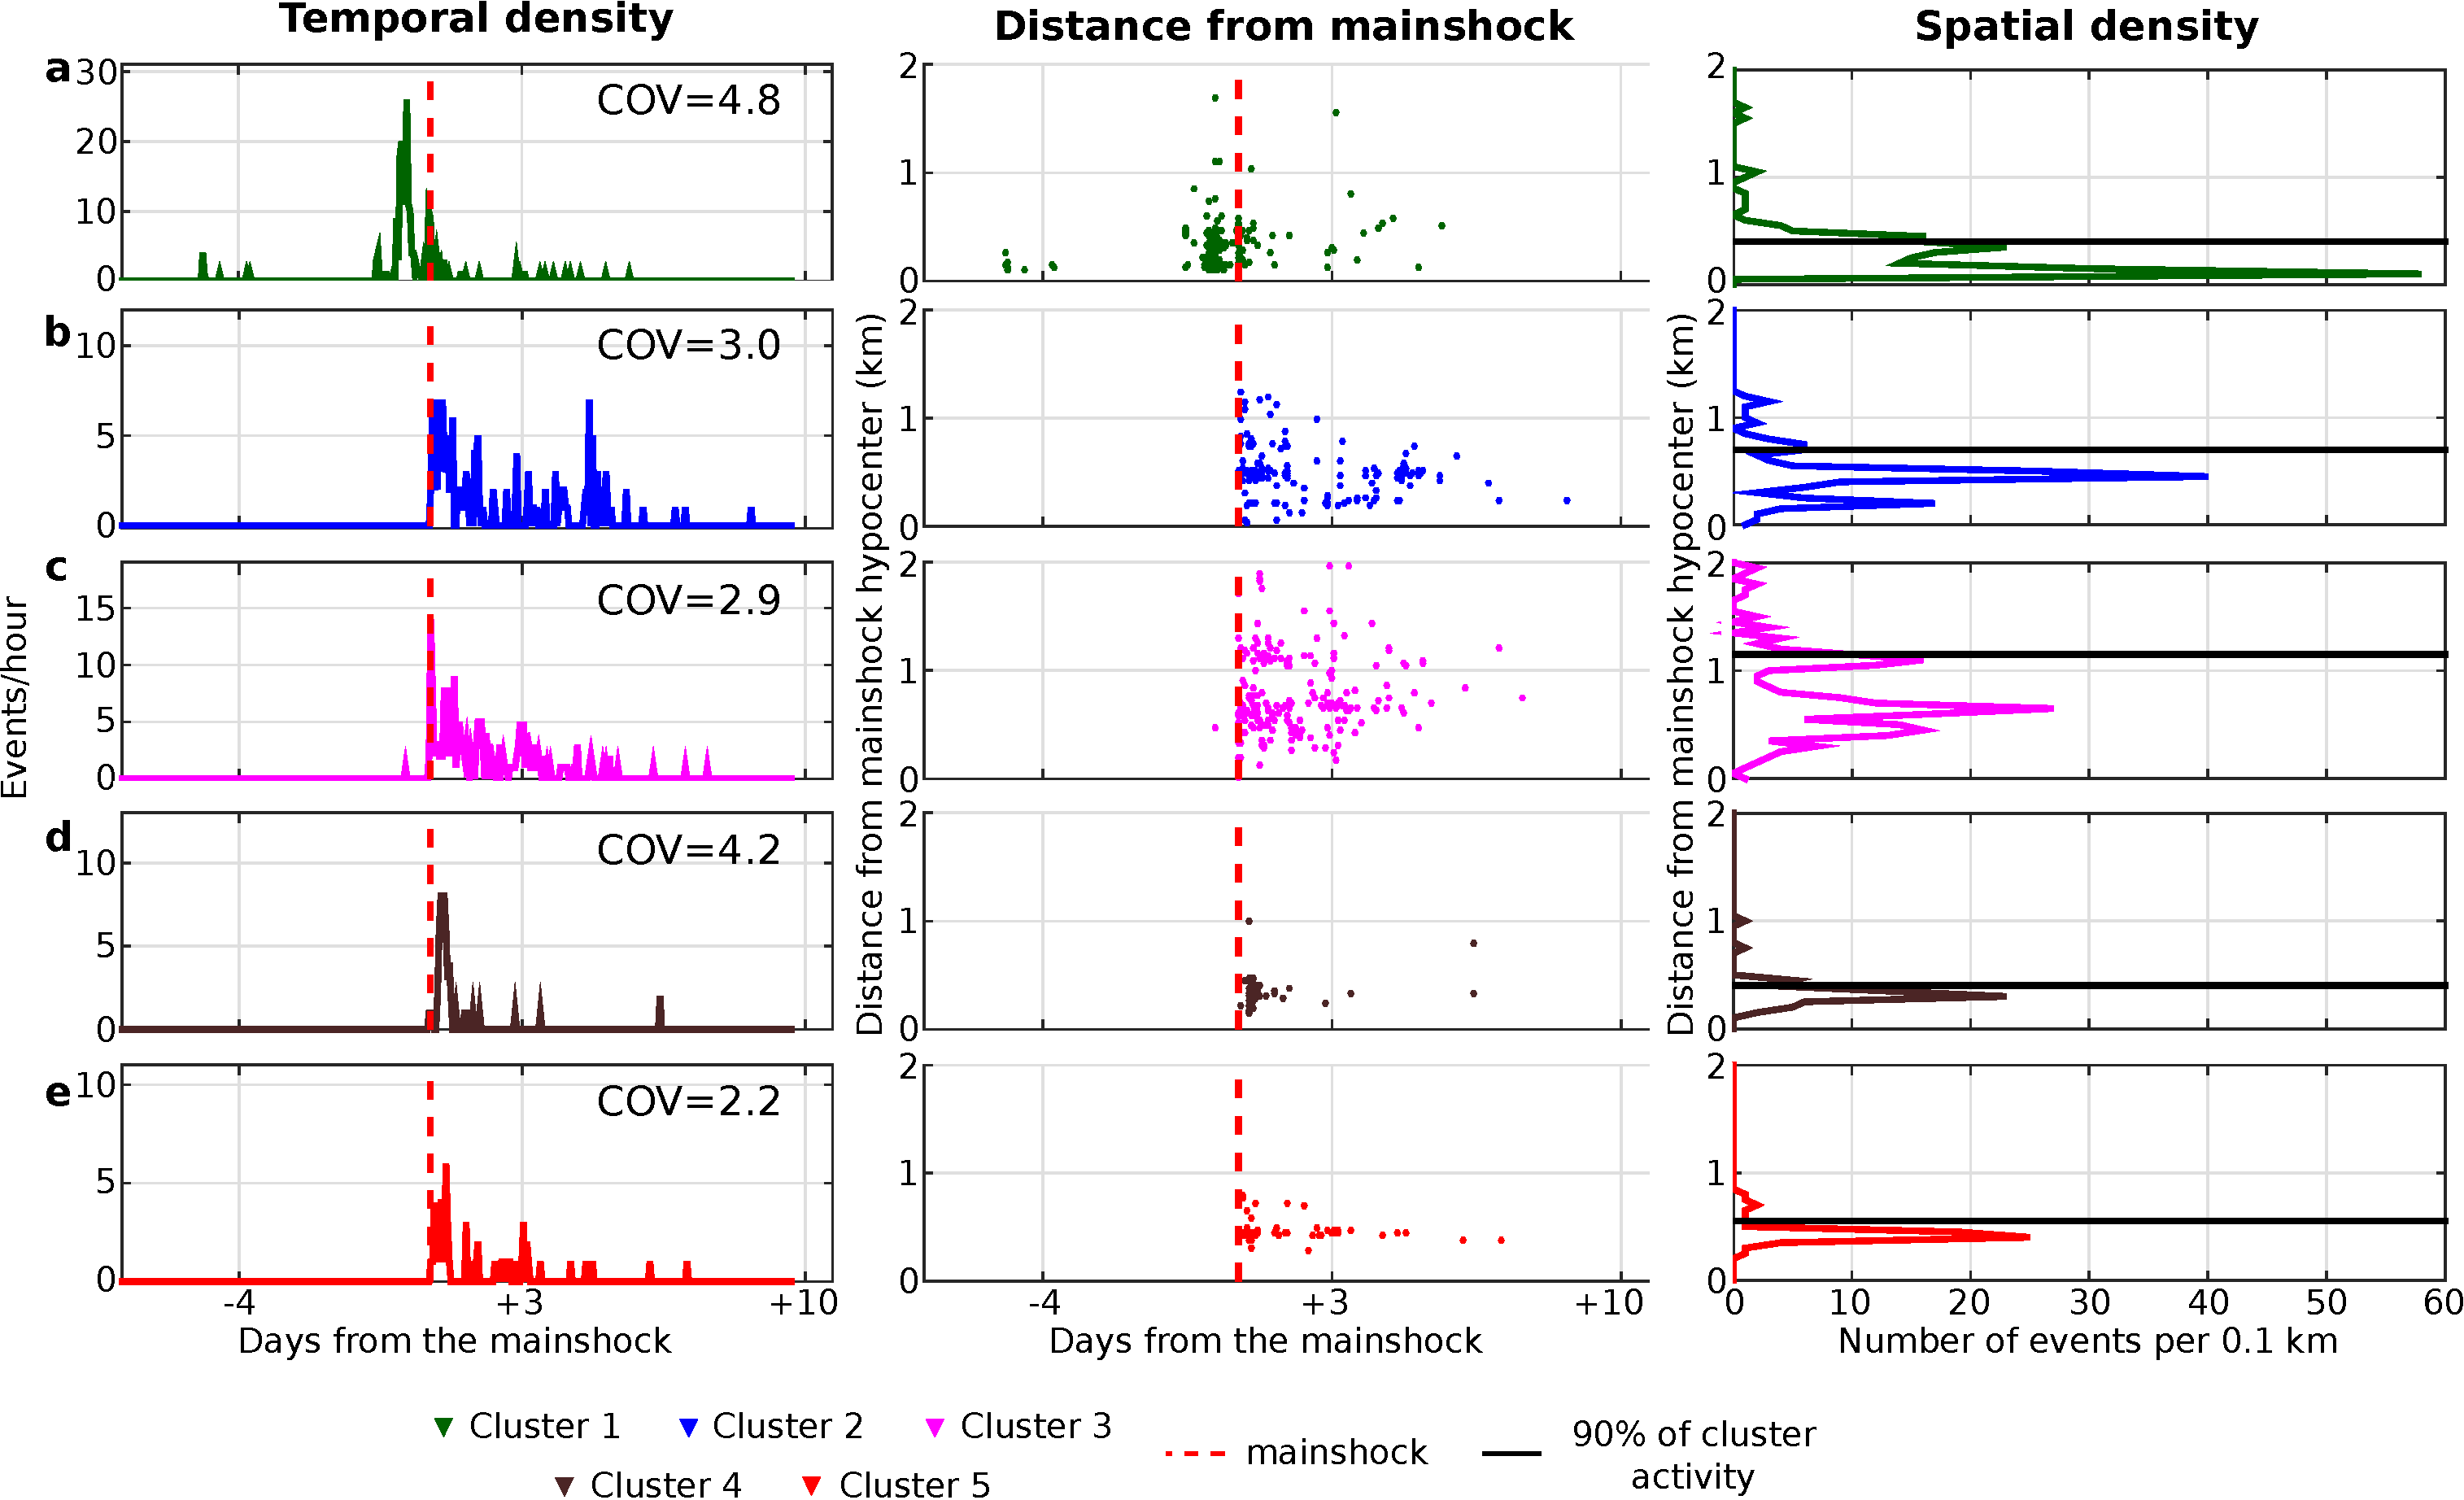
\includegraphics[width=1\linewidth]{densities_plot.pdf}         \caption{Spatio-temporal evolution of the earthquake sequences with respect to the mainshock origin time and hypocenter. Left column: Temporal density (number of events per hour). The coefficients of variation (COV) from the recurrence times are indicated for each cluster. Black dashed line, mainshock hypocenter and origin time. Center column: Distance in time and space from each event of the sequence with respect to the mainshock location and origin time. Black dashed line, mainshock hypocenter and origin time. Right column: Spatial density (concentration of events per 0.1 km). Solid line, where 90\% of the seismic activity is concentrated. (a)-(e) Each of the five clusters. The same color code from Figure 3 is used.}
\end{figure}     \label{fig:time_each_cluster}

\begin{center}
   [Figure 5]
\end{center}

\begin{figure}
    \centering
     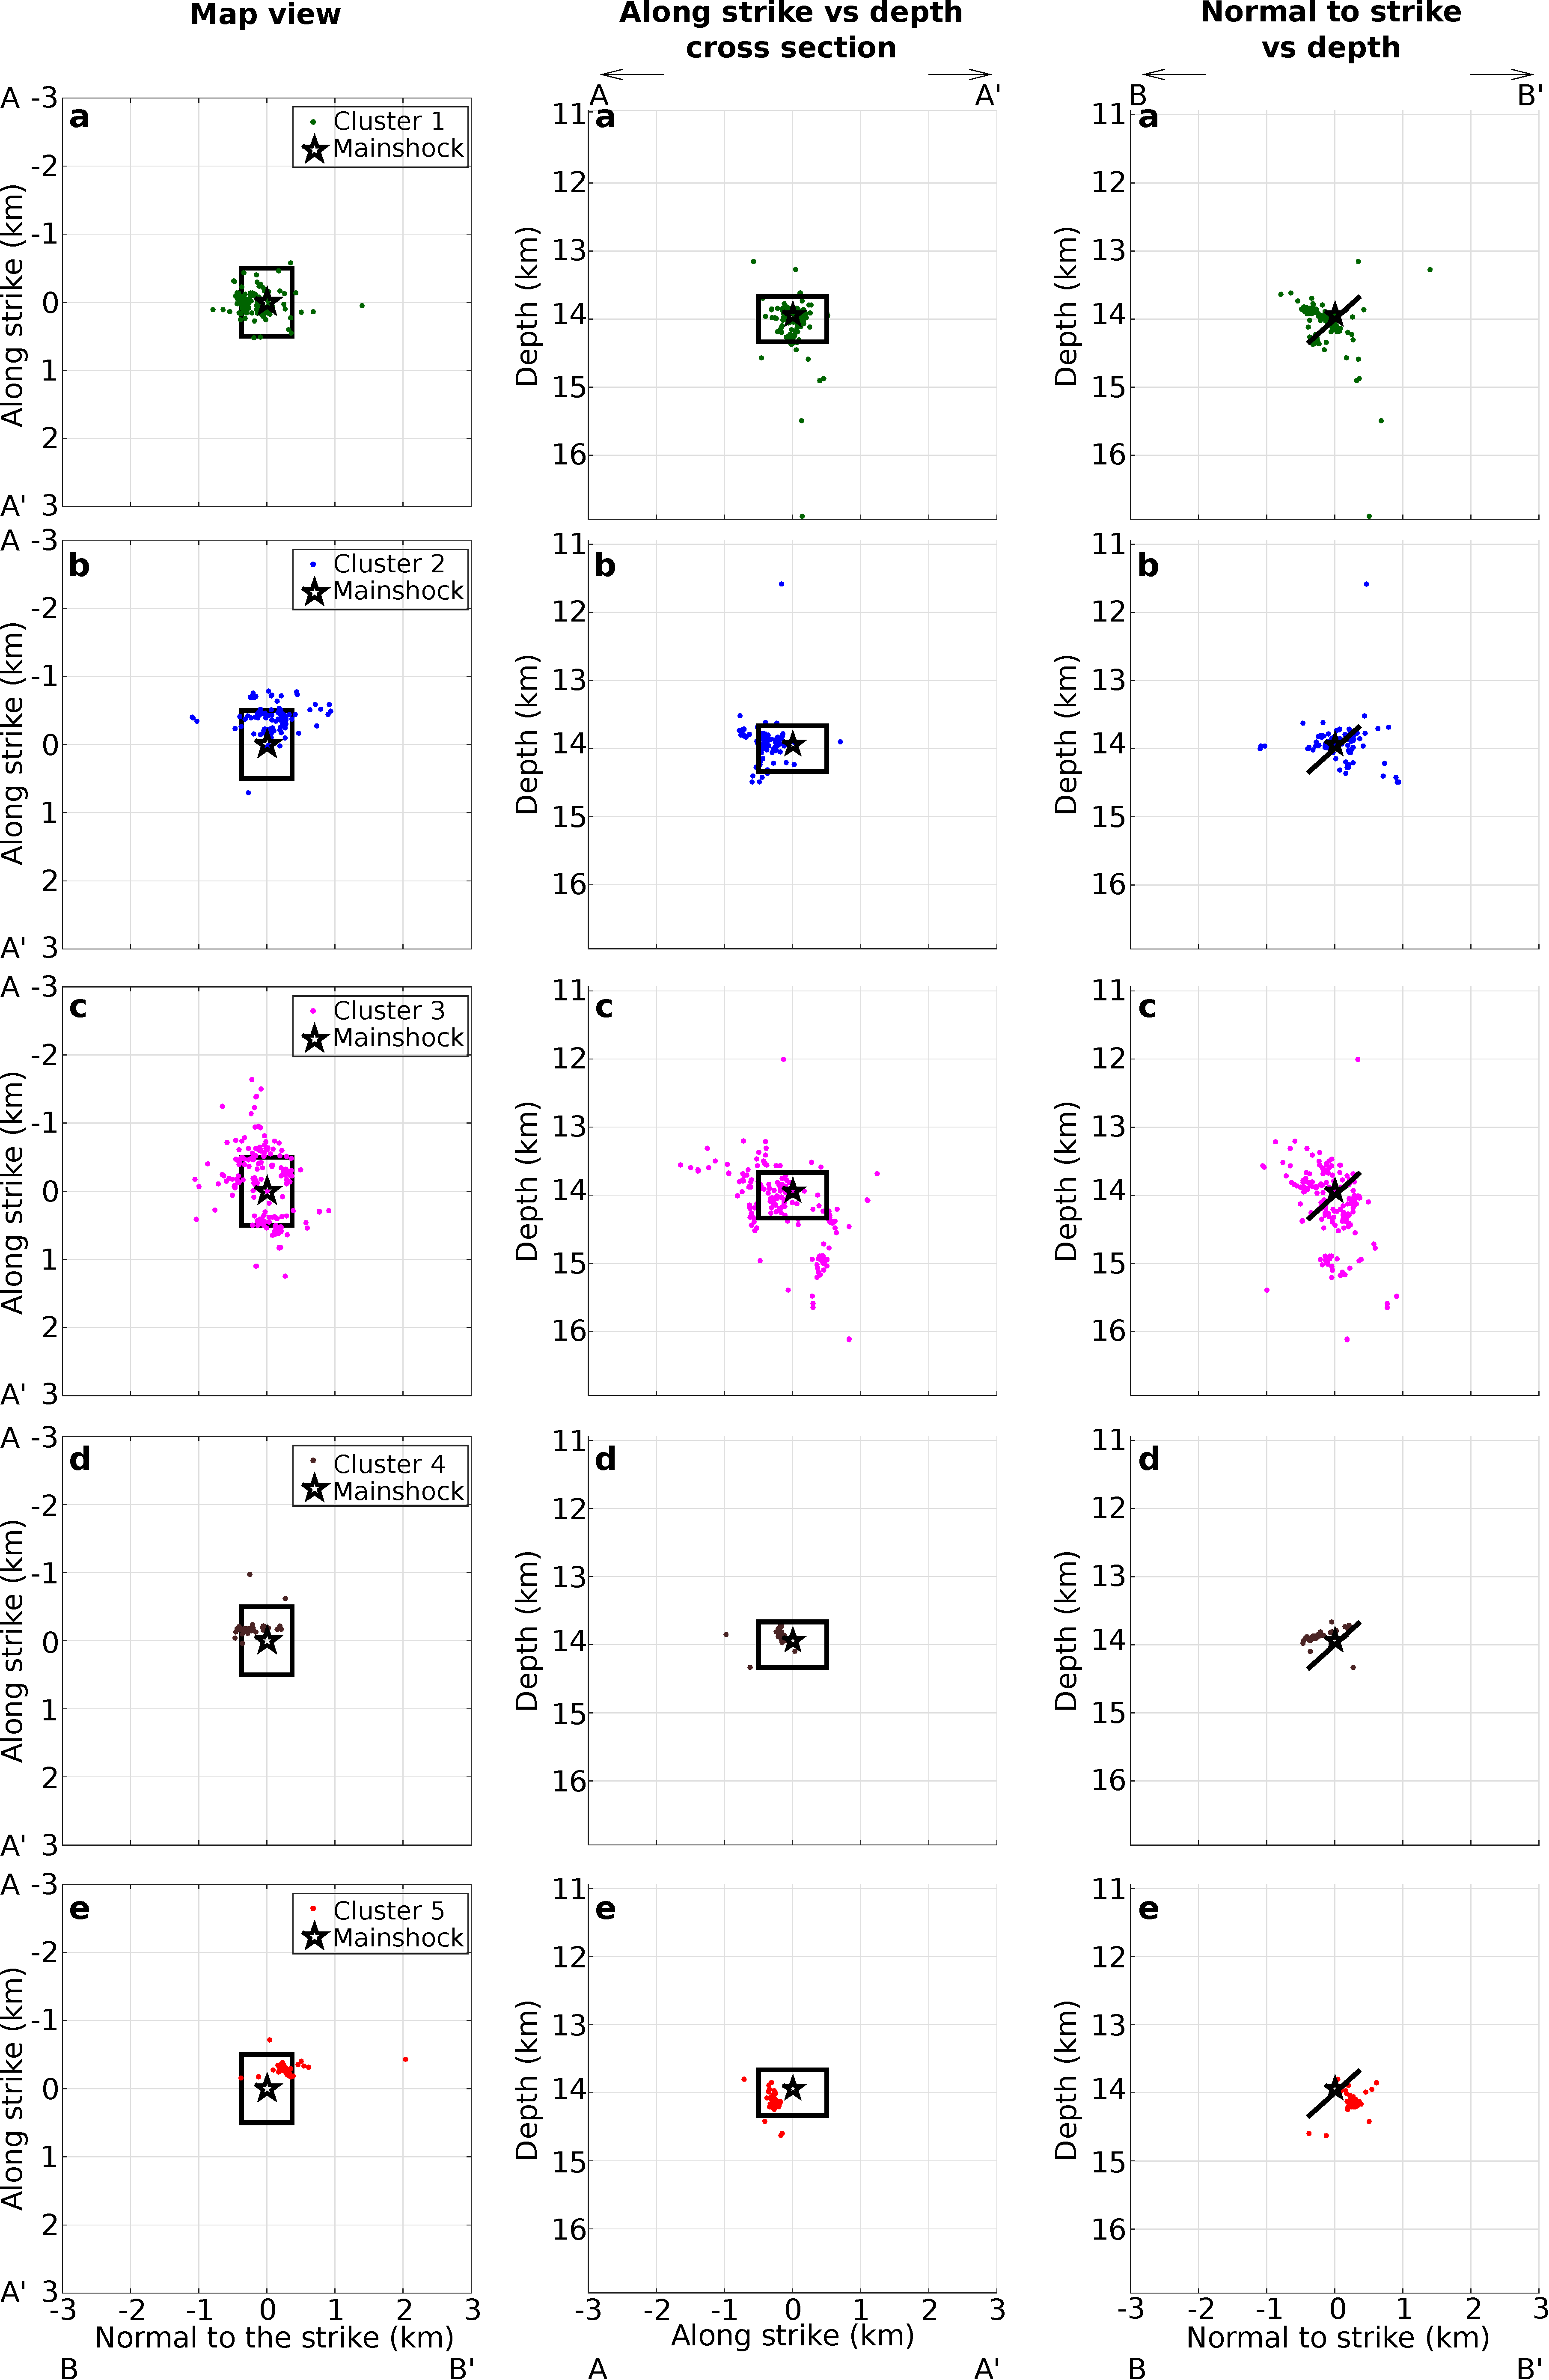
\includegraphics[width=0.9\linewidth]{maps_clusters.pdf}     \caption{Map view (left column), and cross-sections along the strike (middle column) and normal-strike (right column) directions for each of the five clusters identified in the sequence (as indicated). All of the locations are relative to the mainshock hypocenter (41.7746$^o$N 13.6066$^o$E; 13.94 km depth, black star). In all of the panels, the same color code is used as in Figures 3 and 4 to represent each different cluster. The solid black line represents a fault plane of 1 km$^2$ with the geometry of the second nodal plane (Supplementary Materials Table S1). The directions A-A' (along strike) and B-B' (normal to the strike) are the same as in Figure 1.}
\end{figure}          \label{fig:maps_each_cluster}

The results of the spatio-temporal evolution for the identified clusters suggest complex evolution of the seismicity. Two fault planes are activated during the sequence, with foreshocks primarily occurring on the antithetic fault plane (Fig. 5a, cross-section), similarly to part of the foreshock activity that was observed for the L'Aquila normal fault earthquake \citep{Chiaraluce_2011_AAN}. Relying only on our observations, it is hard to unravel which mechanism(s) might be responsible for the occurrence of the foreshocks, and thus the driving of the main event. For example, there are no exponential or power-law increments of events seen while approaching the main event \citep{Papazachos_1975_FEP,Kagan_1978_SSO}, which might suggest accelerating aseismic slip \citep{Dodge_1996_DOC, Bouchon_2011_ENI, Tape_2018_ENF}. Neither are any spatial patterns seen (\emph{e.g.}, migrations) that might suggest the same mechanism, or might alternatively indicate triggering by stress transfer \citep{Dodge_1996_DOC, Ellsworth_2018_NIE, Yoon_2019_FMN}. However, we clearly outline the differences between the foreshocks and aftershocks. In particular, the foreshocks occur in a more temporal clustered manner, and they are closer to the hypocenter of the main event (Fig. 4a). The compact and highly temporal clustered seismicity indicates strong event interactions, and favors stress transfer as the mechanism for foreshock occurrence \citep[COV,][]{Schoenball_2017_SAS}.

Interestingly, the aftershock clusters also show different spatio-temporal behaviors between each other (Figs. 5b-e, 4b-e). The observed differences might be explained by different physical processes driving the aftershock occurrence. For example, the events in clusters 2 and 3 (Fig. 5b,c) spread in a volume around the fault. This spatial pattern is likely to result from stress redistribution, volumetric damage, and relaxation processes after the mainshock \citep{trugman2020imaging}. In contrast, clusters 4 and 5 follow the orientation of the main fault in a more compact volume around it (Fig. 5d,e), and their activity decays in a rapid manner (Fig. 4). This behavior might suggest that these latter clusters result from stress increments induced by the mainshock afterslip that occurs near the fault plane region in the few hours or days after the main event \citep{Stein_1983_HVE, Shen_1994_PDF}.

As in previous studies \citep{Mcmahon_2017_STE, Savage_2017_PPS, Mcmahon2019_STA}, we can see that this detailed analysis of seismic data reveals a complex and imbricated earthquake sequence, for which the mainshock initiation is unlikely to result from only the evolution of physical properties (\emph{e.g.}, stress, friction) on the main fault plane. Indeed the sequence begins through an interaction between the antithetic and main faults during the foreshock-mainshock sequences, similar to that observed for other events \citep{Chiaraluce_2011_AAN, Mcmahon2019_STA}. In normal faults, this behavior can be related to preseismic processes in the dilation wedge located in the hanging wall \citep{Doglion_2011_RBD}. The complexity of the sequence might also emerge from fluid involvement, which is known to have a significant role in the control of seismicity and its 'style' in the central Apennines \citep{antonioli2005fluid, poliseasonal}. The stress perturbations in the antithetic fault might have modified the local pore pressures, with fluid migration into the main fault, which would favor the occurrence of the main event \citep{Doglion_2011_RBD}. 

\section*{Conclusion}

By using a combination of high-resolution detection methods, precise relocation \citep[\emph{e.g.},][]{Gibbons_2006_DLM, Waldhauser_2001_HDD} and waveform clustering, we have unveiled the complexity of the sequences associated with the 2019 (M$_w$ 4.4) Balsorano earthquake. We detect 714 events that comprise this sequence. These events are classified into five different seismic clusters. The differences between these clusters are highlighted by their distinct spatio-temporal properties that are unveiled by the waveform-based clustering analysis \citep{Kagan_1991_LTE, wehling_2013_IDT, Cesca_2014_SMC, Ellsworth_2018_NIE}, and by their relative source locations \citep{Waldhauser_2001_HDD}.

Our results highlight different behaviors between foreshocks and aftershocks. For example, foreshocks occur in a compact region near the mainshock hypocenter, and show high temporal clustering  (Fig. 4a). The lack of repeating events (\emph{i.e.}, highly correlated events with correlation coefficient $>$0.9), strong temporal clustering, and inter-event proximity might indicate that stress transfer triggering has the main role in driving the occurrence of the foreshocks \citep{Dodge_1996_DOC}. Nevertheless, there are no observations that can exclude aseismic slip. The foreshock activity mainly take place in an antithetic fault (Fig. 5a), which suggests that the initiation processes do not only occur on one fault plane, but involve larger volumes \citep{Savage_2017_PPS}. This precursory antithetic activation has been observed in other normal fault events \citep{Chiaraluce_2011_AAN} and it can be expected in some gravity-driven normal fault models \citep{Doglion_2011_RBD}. 

Furthermore, our analysis shows diversity for the aftershocks behavior. Indeed, four different clusters comprise the aftershock sequences. Two of these four are spread in a volume around the main fault (Fig. 5b,c), and might result from stress redistribution after the mainshock (\emph{e.g.}, caused by volumetric damage and the relaxation processes; \cite{trugman2020imaging}). Given the rapid temporal decay of their activity and their compactness and spatial orientation, the remaining two clusters appear to be driven by rapid stress increments induced by the mainshock and afterslip that occur near the fault plane in the few days after the mainshock \citep{Stein_1983_HVE, Shen_1994_PDF}.

In summary, this study of foreshocks and aftershocks highlights that simple preparation models with evolution of stress and friction on a single fault plane are not suited to precisely explain the evolution of the seismicity we observe here for a real fault. A relatively large volume appears to be involved in the earthquake initiation, over a short time scale ($\sim$1 day). We further highlight how the full range of aftershocks is likely to be an ensemble average view of different processes, which will include afterslip, volumetric damage, and relaxation. Continuing to provide detailed information about foreshocks and their relationships to the mainshock and aftershocks also for relatively small events can help us to develop new and more realistic models that can provide better fitting of seismological observations and shed new light on the initiation of earthquakes in real faults.


\section*{Data and resources}

The continuous seismic data used in this study are available at the Istituto Nazionale di Geofisica e Vulcanologia (INGV) seismological data center (\href{http://cnt.rm.ingv.it/webservices_and_software/}{\color{blue}http://cnt.rm.ingv.it/webservices\_and\_software/}; last accessed, March 2020) and were downloaded using obspyDMT (\href{https://github.com/kasra-hosseini/obspyDMT}{\color{blue}https://github.com/kasra-hosseini/obspyDMT}, \cite{Hosseini_2017_obspyDMT}). The fast matched filter \citep{Beauce_2017_FMF} used in this study can be found at \href{https://github.com/beridel/fast_matched_filter}{\color{blue}https://github.com/beridel/fast\_matched\_filter}. Some plots were made using the Generic Mapping Tools version 4.5.14 (\href{www.soest.hawaii.edu/gmt}{\color{blue}www.soest.hawaii.edu/gmt}; \cite{Wessel_1998_NIV}). The event clustering was performed using Scikit-learn (\href{https://scikit-learn.org/stable/}{https://scikit-learn.org/stable/}; \cite{scikit-learn})

\section*{Acknowledgments}

This research received funding from the European Research Council (ERC) under the European Union   Horizon 2020 Research and Innovation Programme (grant  agreement 802777-MONIFAULTS). Computations were performed using the Univertity of Grenoble Alpes (UGA) High-Performance Computing infrastructures CIMENT \\ \noindent (\href{https://ciment.univ-grenoble-alpes.fr}{\color{blue}https://ciment.univ-grenoble-alpes.fr}). 

%\bibliography{bibliography}
%\bibliographystyle{apalike}

\begin{thebibliography}{}

\bibitem[Abercrombie and Mori, 1996]{Abercrombie_1996_OPF}
Abercrombie, R.~E. and Mori, J. (1996).
\newblock Occurrence patterns of foreshocks to large earthquakes in the western
  united states.
\newblock {\em Nature}, 381(6580):303--307.

\bibitem[Antonioli et~al., 2005]{antonioli2005fluid}
Antonioli, A., Piccinini, D., Chiaraluce, L., and Cocco, M. (2005).
\newblock Fluid flow and seismicity pattern: Evidence from the 1997
  umbria-marche (central italy) seismic sequence.
\newblock {\em Geophysical Research Letters}, 32(10).

\bibitem[Bagh et~al., 2007]{Bagh_2007_BSC}
Bagh, S., Chiaraluce, L., De~Gori, P., Moretti, M., Govoni, A., Chiarabba, C.,
  Di~Bartolomeo, P., and Romanelli, M. (2007).
\newblock Background seismicity in the central apennines of italy: The abruzzo
  region case study.
\newblock {\em Tectonophysics}, 444(1-4):80--92.

\bibitem[Beauc\'e et~al., 2017]{Beauce_2017_FMF}
Beauc\'e, E., Frank, W.~B., and Romanenko, A. (2017).
\newblock Fast matched filter (fmf): An efficient seismic matched-filter search
  for both cpu and gpu architectures.
\newblock {\em Seismological Research Letters}, 89(1):165.

\bibitem[Bouchon et~al., 2013]{Bouchon_2013_LPP}
Bouchon, M., Durand, V., Marsan, D., Karabulut, H., and Schmittbuhl, J. (2013).
\newblock The long precursory phase of most large interplate earthquakes.
\newblock {\em Nature geoscience}, 6(4):299--302.

\bibitem[Bouchon et~al., 2011]{Bouchon_2011_ENI}
Bouchon, M., Karabulut, H., Aktar, M., {\"O}zalaybey, S., Schmittbuhl, J., and
  Bouin, M.-P. (2011).
\newblock Extended nucleation of the 1999 mw 7.6 izmit earthquake.
\newblock {\em science}, 331(6019):877--880.

\bibitem[Brune, 1979]{Brune_1979_IET}
Brune, J.~N. (1979).
\newblock Implications of earthquake triggering and rupture propagation for
  earthquake prediction based on premonitory phenomena.
\newblock {\em Journal of Geophysical Research: Solid Earth},
  84(B5):2195--2198.

\bibitem[Cattaneo et~al., 1999]{Cattaneo_1999_WSA}
Cattaneo, M., Augliera, P., Spallarossa, D., and Lanza, V. (1999).
\newblock A waveform similarity approach to investigate seismicity patterns.
\newblock {\em Natural hazards}, 19(2-3):123--138.

\bibitem[Cesca et~al., 2014]{Cesca_2014_SMC}
Cesca, S., {\c{S}}en, A.~T., and Dahm, T. (2014).
\newblock Seismicity monitoring by cluster analysis of moment tensors.
\newblock {\em Geophysical Journal International}, 196(3):1813--1826.

\bibitem[Chen and Shearer, 2013]{Chen_2013_CFS}
Chen, X. and Shearer, P.~M. (2013).
\newblock California foreshock sequences suggest aseismic triggering process.
\newblock {\em Geophysical Research Letters}, 40(11):2602--2607.

\bibitem[Chiaraluce et~al., 2011]{Chiaraluce_2011_AAN}
Chiaraluce, L., Valoroso, L., Piccinini, D., Di~Stefano, R., and De~Gori, P.
  (2011).
\newblock The anatomy of the 2009 l'aquila normal fault system (central italy)
  imaged by high resolution foreshock and aftershock locations.
\newblock {\em Journal of Geophysical Research: Solid Earth}, 116(B12).

\bibitem[D'agostino et~al., 2001]{Dagostino_2001a_ACE}
D'agostino, N., Giuliani, R., Mattone, M., and Bonci, L. (2001).
\newblock Active crustal extension in the central apennines (italy) inferred
  from gps measurements in the interval 1994--1999.
\newblock {\em Geophysical Research Letters}, 28(10):2121--2124.

\bibitem[De~Santis et~al., 2019]{DeSantins_2019_PWS}
De~Santis, A., Marchetti, D., Pav\'on-Carrasco, F.~J., Cianchini, G.,
  Perrone, L., Abbattista, C., Alfonsi, L., Amoruso, L., Campuzano, S.~A.,
  Carbone, M., et~al. (2019).
\newblock Precursory worldwide signatures of earthquake occurrences on swarm
  satellite data.
\newblock {\em Scientific reports}, 9(1):1--13.

\bibitem[Dieterich, 1994]{Dieterich_1994_CLR}
Dieterich, J. (1994).
\newblock A constitutive law for rate of earthquake production and its
  application to earthquake clustering.
\newblock {\em Journal of Geophysical Research: Solid Earth},
  99(B2):2601--2618.

\bibitem[Dieterich, 1992]{Dieterich_1992_ENF}
Dieterich, J.~H. (1992).
\newblock Earthquake nucleation on faults with rate-and state-dependent
  strength.
\newblock {\em Tectonophysics}, 211(1-4):115--134.

\bibitem[Dodge et~al., 1996]{Dodge_1996_DOC}
Dodge, D.~A., Beroza, G.~C., and Ellsworth, W. (1996).
\newblock Detailed observations of california foreshock sequences: Implications
  for the earthquake initiation process.
\newblock {\em Journal of Geophysical Research: Solid Earth},
  101(B10):22371--22392.

\bibitem[Doglioni et~al., 2011]{Doglion_2011_RBD}
Doglioni, C., Barba, S., Carminati, E., and Riguzzi, F. (2011).
\newblock Role of the brittle--ductile transition on fault activation.
\newblock {\em Physics of the Earth and Planetary Interiors},
  184(3-4):160--171.

\bibitem[Dublanchet, 2018]{dublanchet2018dynamics}
Dublanchet, P. (2018).
\newblock The dynamics of earthquake precursors controlled by effective
  friction.
\newblock {\em Geophysical Journal International}, 212(2):853--871.
  
\bibitem[Eftaxias et~al., 2000]{Eftaxias_2000_DEE}
Eftaxias, K., Kopanas, J., Bogris, N., KAPIRIS, P., ANTONOPOULOS, G., and
  VAROTSOS, P. (2000).
\newblock Detection of electromagnetic earthquake precursory signals in greece.
\newblock {\em Proceedings of the Japan Academy, Series B}, 76(4):45--50.

\bibitem[Ellsworth and Beroza, 1995]{Ellsworth_1995_SEE}
Ellsworth, W.~L. and Beroza, G.~C. (1995).
\newblock Seismic evidence for an earthquake nucleation phase.
\newblock {\em Science}, 268(5212):851--855.

\bibitem[Ellsworth and Bulut, 2018]{Ellsworth_2018_NIE}
Ellsworth, W.~L. and Bulut, F. (2018).
\newblock Nucleation of the 1999 izmit earthquake by a triggered cascade of
  foreshocks.
\newblock {\em Nature Geoscience}, 11(7):531--535.

\bibitem[Felzer et~al., 2004]{Felzer_2004_COA}
Felzer, K.~R., Abercrombie, R.~E., and Ekstrom, G. (2004).
\newblock A common origin for aftershocks, foreshocks, and multiplets.
\newblock {\em Bulletin of the Seismological Society of America}, 94(1):88--98.

\bibitem[Gibbons and Ringdal, 2006]{Gibbons_2006_DLM}
Gibbons, S.~J. and Ringdal, F. (2006).
\newblock The detection of low magnitude seismic events using array-based
  waveform correlation.
\newblock {\em Geophysical Journal International}, 165(1):149--166.

\bibitem[Goebel et~al., 2012]{Goebel_2012_IFH}
Goebel, T., Becker, T., Schorlemmer, D., Stanchits, S., Sammis, C., Rybacki,
  E., and Dresen, G. (2012).
\newblock Identifying fault heterogeneity through mapping spatial anomalies in
  acoustic emission statistics.
\newblock {\em Journal of Geophysical Research: Solid Earth}, 117(B3).

\bibitem[Hosseini and Sigloch, 2017]{Hosseini_2017_obspyDMT}
Hosseini, K. and Sigloch, K. (2017).
\newblock Obspydmt: a python toolbox for retrieving and processing large
  seismological data sets.
\newblock {\em Solid Earth}, (5):1047--1070.

\bibitem[Hunstad and England, 1999]{Hunstad_1999_UBR}
Hunstad, I. and England, P. (1999).
\newblock An upper bound on the rate of strain in the central apennines, italy,
  from triangulation measurements between 1869 and 1963.
\newblock {\em Earth and Planetary Science Letters}, 169(3-4):261--267.

\bibitem[Jones and Molnar, 1979]{Jones_1979_SCF}
Jones, L.~M. and Molnar, P. (1979).
\newblock Some characteristics of foreshocks and their possible relationship to
  earthquake prediction and premonitory slip on faults.
\newblock {\em Journal of Geophysical Research: Solid Earth},
  84(B7):3596--3608.

\bibitem[Jones, 1985]{Jones_1985_FTE}
Jones, L.~M. (1985).
\newblock Foreshocks and time-dependent earthquake hazard assessment in
  southern california.
\newblock {\em Bulletin of the Seismological Society of America},
  75(6):1669--1679.

\bibitem[Kagan and Jackson, 1991]{Kagan_1991_LTE}
Kagan, Y. and Jackson, D.~D. (1991).
\newblock Long-term earthquake clustering.
\newblock {\em Geophysical Journal International}, 104(1):117--133.

\bibitem[Kagan and Knopoff, 1978]{Kagan_1978_SSO}
Kagan, Y. and Knopoff, L. (1978).
\newblock Statistical study of the occurrence of shallow earthquakes.
\newblock {\em Geophysical Journal International}, 55(1):67--86.
  
\bibitem[Kato et~al., 2012]{Kato_2012_PSS}
Kato, A., Obara, K., Igarashi, T., Tsuruoka, H., Nakagawa, S., and Hirata, N.
  (2012).
\newblock Propagation of slow slip leading up to the 2011 mw 9.0 tohoku-oki
  earthquake.
\newblock {\em Science}, 335(6069):705--708.

\bibitem[Liu and Rice, 2005]{Liu_2005_AST}
Liu, Y. and Rice, J.~R. (2005).
\newblock Aseismic slip transients emerge spontaneously in three-dimensional
  rate and state modeling of subduction earthquake sequences.
\newblock {\em Journal of Geophysical Research: Solid Earth}, 110(B8).

\bibitem[Malin et~al., 2018]{Malin_2018_MPE}
Malin, P.~E., Bohnhoff, M., Bl{\"u}mle, F., Dresen, G.,
  Mart{\'\i}nez-Garz{\'o}n, P., Nurlu, M., Ceken, U., Kadirioglu, F.~T.,
  Kartal, R.~F., Kilic, T., et~al. (2018).
\newblock Microearthquakes preceding a m4. 2 earthquake offshore istanbul.
\newblock {\em Scientific reports}, 8(1):1--11.

\bibitem[Marone, 1998]{Marone_1998_ELR}
Marone, C. (1998).
\newblock The effect of loading rate on static friction and the rate of fault
  healing during the earthquake cycle.
\newblock {\em Nature}, 391(6662):69--72.

\bibitem[McLaskey, 2019]{mclaskey2019earthquake}
McLaskey, G.~C. (2019).
\newblock Earthquake initiation from laboratory observations and implications
  for foreshocks.
\newblock {\em Journal of Geophysical Research: Solid Earth}.

\bibitem[McMahon et~al., 2017]{Mcmahon_2017_STE}
McMahon, N.~D., Aster, R.~C., Yeck, W.~L., McNamara, D.~E., and Benz, H.~M.
  (2017).
\newblock Spatiotemporal evolution of the 2011 prague, oklahoma, aftershock
  sequence revealed using subspace detection and relocation.
\newblock {\em Geophysical Research Letters}, 44(14):7149--7158.

\bibitem[McMahon et~al., 2019]{Mcmahon2019_STA}
McMahon, N.~D., Yeck, W.~L., Stickney, M.~C., Aster, R.~C., Martens, H.~R., and
  Benz, H.~M. (2019).
\newblock Spatiotemporal analysis of the foreshock--mainshock--aftershock
  sequence of the 6 july 2017 m w 5.8 lincoln, montana, earthquake.
\newblock {\em Seismological Research Letters}, 90(1):131--139.

\bibitem[Mignan, 2014]{Mignan_2014_DPV}
Mignan, A. (2014).
\newblock The debate on the prognostic value of earthquake foreshocks: A
  meta-analysis.
\newblock {\em Scientific reports}, 4:4099.

\bibitem[Mogi, 1963]{Mogi_1963_SDA}
Mogi, K. (1963).
\newblock Some discussions on aftershocks, foreshocks and earthquake swarms:
  the fracture of a semi-infinite body caused by an inner stress origin and its
  relation to the earthquake phenomena (third paper).
\newblock {\em Bulletin of the Earthquake
  Research Institute, University of Tokyo}, 41(3):615--658.

\bibitem[Molchanov et~al., 1998]{Molchanov_1998_PES}
Molchanov, O., Hayakawa, M., Oudoh, T., and Kawai, E. (1998).
\newblock Precursory effects in the subionospheric vlf signals for the kobe
  earthquake.
\newblock {\em Physics of the Earth and Planetary Interiors},
  105(3-4):239--248.
  
\bibitem[Papazachos, 1975]{Papazachos_1975_FEP}
Papazachos, B. (1975).
\newblock Foreshocks and earthquake prediction.
\newblock {\em Tectonophysics}, 28(4):213--226.

\bibitem[Pedregosa et~al., 2011]{scikit-learn}
Pedregosa, F., Varoquaux, G., Gramfort, A., Michel, V., Thirion, B., Grisel,
  O., Blondel, M., Prettenhofer, P., Weiss, R., Dubourg, V., Vanderplas, J.,
  Passos, A., Cournapeau, D., Brucher, M., Perrot, M., and Duchesnay, E.
  (2011).
\newblock Scikit-learn: Machine learning in {P}ython.
\newblock {\em Journal of Machine Learning Research}, 12:2825--2830.

\bibitem[Poli et~al., 020a]{poliseasonal}
Poli, P., Marguin, V., Wang, Q., D’agostino, N., and Johnson, P. (2020a).
\newblock Seasonal and co-seismic velocity variation in the region of
  l’aquila from single station measurements and implications for crustal
  rheology.
\newblock {\em Journal of Geophysical Research: Solid Earth}, page
  e2019JB019316.

\bibitem[Poli et~al., 020b]{Poli_2020}
Poli, P., Soaga, J., Molinari, I., Cascone, V., and Boschi, L. (2020b).
\newblock The 2020 coronavirus lockdown and seismic monitoring of anthropic
  activities in northern italy.
\newblock {\em Sci Rep}, 10:--.
  
\bibitem[Reasenberg, 1999]{Reasenberg_1999_FOB}
Reasenberg, P.~A. (1999).
\newblock Foreshock occurrence before large earthquakes.
\newblock {\em Journal of Geophysical Research: Solid Earth},
  104(B3):4755--4768.
  
\bibitem[Renard et~al., 2019]{Renard_2019_VSP}
Renard, F., McBeck, J., Kandula, N., Cordonnier, B., Meakin, P., and Ben-Zion,
  Y. (2019).
\newblock Volumetric and shear processes in crystalline rock approaching
  faulting.
\newblock {\em Proceedings of the National Academy of Sciences},
  116(33):16234--16239.

\bibitem[Rikitake, 1975]{Rikitake_1975_EP}
Rikitake, T. (1975).
\newblock Earthquake precursors.
\newblock {\em Bulletin of the Seismological Society of America},
  65(5):1133--1162.
  
\bibitem[Roberts and Michetti, 2004]{Roberts_2004_STV}
Roberts, G.~P. and Michetti, A.~M. (2004).
\newblock Spatial and temporal variations in growth rates along active normal
  fault systems: an example from the lazio--abruzzo apennines, central italy.
\newblock {\em Journal of Structural Geology}, 26(2):339--376.

\bibitem[Rubin and Ampuero, 2005]{Rubin_2005_ENR}
Rubin, A.~M. and Ampuero, J.-P. (2005).
\newblock Earthquake nucleation on (aging) rate and state faults.
\newblock {\em Journal of Geophysical Research: Solid Earth}, 110(B11).

\bibitem[Ruiz et~al., 2017]{ruiz2017nucleation}
Ruiz, S., Aden-Antoniow, F., Baez, J., Otarola, C., Potin, B., del Campo, F.,
  Poli, P., Flores, C., Satriano, C., Leyton, F., et~al. (2017).
\newblock Nucleation phase and dynamic inversion of the mw 6.9 valpara{\'\i}so
  2017 earthquake in central chile.
\newblock {\em Geophysical Research Letters}, 44(20):10--290.

\bibitem[Ruiz et~al., 2014a]{ruiz2014intense}
Ruiz, S., Metois, M., Fuenzalida, A., Ruiz, J., Leyton, F., Grandin, R., Vigny,
  C., Madariaga, R., and Campos, J. (2014a).
\newblock Intense foreshocks and a slow slip event preceded the 2014 iquique mw
  8.1 earthquake.
\newblock {\em Science}, 345(6201):1165--1169.

\bibitem[Ruiz et~al., 2014b]{Ruiz_2014_IFS}
Ruiz, S., Metois, M., Fuenzalida, A., Ruiz, J., Leyton, F., Grandin, R., Vigny,
  C., Madariaga, R., and Campos, J. (2014b).
\newblock Intense foreshocks and a slow slip event preceded the 2014 iquique mw
  8.1 earthquake.
\newblock {\em Science}, 345(6201):1165--1169.

\bibitem[Savage et~al., 2017]{Savage_2017_PPS}
Savage, H.~M., Keranen, K.~M., P.~Schaff, D., and Dieck, C. (2017).
\newblock Possible precursory signals in damage zone foreshocks.
\newblock {\em Geophysical Research Letters}, 44(11):5411--5417.

\bibitem[Schoenball and Ellsworth, 2017]{Schoenball_2017_SAS}
Schoenball, M. and Ellsworth, W.~L. (2017).
\newblock A systematic assessment of the spatiotemporal evolution of fault
  activation through induced seismicity in oklahoma and southern kansas.
\newblock {\em Journal of Geophysical Research: Solid Earth}, 122(12):10--189.

\bibitem[Schurr et~al., 2014]{Schurr_2014_GUP}
Schurr, B., Asch, G., Hainzl, S., Bedford, J., Hoechner, A., Palo, M., Wang,
  R., Moreno, M., Bartsch, M., Zhang, Y., et~al. (2014).
\newblock Gradual unlocking of plate boundary controlled initiation of the 2014
  iquique earthquake.
\newblock {\em Nature}, 512(7514):299--302.

\bibitem[Shelly et~al., 2007]{Shelly_2007_CET}
Shelly, D.~R., Beroza, G.~C., and Ide, S. (2007).
\newblock Complex evolution of transient slip derived from precise tremor
  locations in western shikoku, japan.
\newblock {\em Geochemistry, Geophysics, Geosystems}, 8(10).

\bibitem[Shelly and Hardebeck, 2019]{Shelly_2019_IFC}
Shelly, D.~R. and Hardebeck, J.~L. (2019).
\newblock Illuminating faulting complexity of the 2017 yellowstone maple creek
  earthquake swarm.
\newblock {\em Geophysical Research Letters}, 46(5):2544--2552.

\bibitem[Shen et~al., 1994]{Shen_1994_PDF}
Shen, Z.-K., Jackson, D.~D., Feng, Y., Cline, M., Kim, M., Fang, P., and Bock,
  Y. (1994).
\newblock Postseismic deformation following the landers earthquake, california,
  28 june 1992.
\newblock {\em Bulletin of the Seismological Society of America},
  84(3):780--791.

\bibitem[Singh et~al., 2010]{Singh_2010_PSU}
Singh, R.~P., Mehdi, W., Gautam, R., Senthil~Kumar, J., Zlotnicki, J., and
  Kafatos, M. (2010).
\newblock Precursory signals using satellite and ground data associated with
  the wenchuan earthquake of 12 may 2008.
\newblock {\em International Journal of Remote Sensing}, 31(13):3341--3354.

\bibitem[Stein and Lisowski, 1983]{Stein_1983_HVE}
Stein, R.~S. and Lisowski, M. (1983).
\newblock The 1979 homestead valley earthquake sequence, california: Control of
  aftershocks and postseismic deformation.
\newblock {\em Journal of Geophysical Research: Solid Earth},
  88(B8):6477--6490.

\bibitem[Tape et~al., 2018]{Tape_2018_ENF}
Tape, C., Holtkamp, S., Silwal, V., Hawthorne, J., Kaneko, Y., Ampuero, J.~P.,
  Ji, C., Ruppert, N., Smith, K., and West, M.~E. (2018).
\newblock Earthquake nucleation and fault slip complexity in the lower crust of
  central alaska.
\newblock {\em Nature Geoscience}, 11(7):536--541.

\bibitem[Tramutoli et~al., 2015]{Tramutoli_2015_VCR}
Tramutoli, V., Corrado, R., Filizzola, C., Genzano, N., Lisi, M., and Pergola,
  N. (2015).
\newblock From visual comparison to robust satellite techniques: 30 years of
  thermal infrared satellite data analyses for the study of earthquake
  preparation phases.
\newblock {\em Bollettino di Geofisica Teorica ed Applicata}, 56(2).


\bibitem[Trugman et~al., 2020]{trugman2020imaging}
Trugman, D.~T., Ross, Z.~E., and Johnson, P.~A. (2020).
\newblock Imaging stress and faulting complexity through earthquake waveform
  similarity.
\newblock {\em Geophysical Research Letters}, 47(1):e2019GL085888.

\bibitem[Virk and Walia, 2001]{Virk_2001_HRP}
Virk, H. and Walia, V. (2001).
\newblock Helium/radon precursory signals of chamoli earthquake, india.
\newblock {\em Radiation measurements}, 34(1-6):379--384.

\bibitem[Waldhauser, 2001]{Waldhauser_2001_HDD}
Waldhauser, F. (2001).
\newblock hypodd—a program to compute double-difference hypocenter locations
  (hypodd version 1.0-03/2001).
\newblock {\em US Geol. Surv. Open File Rep., 01}, 113.

\bibitem[Ward~Jr, 1963]{Ward_1963_HGO}
Ward~Jr, J.~H. (1963).
\newblock Hierarchical grouping to optimize an objective function.
\newblock {\em Journal of the American statistical association},
  58(301):236--244.

\bibitem[Wehling-Benatelli et~al., 2013]{wehling_2013_IDT}
Wehling-Benatelli, S., Becker, D., Bischoff, M., Friederich, W., and Meier, T.
  (2013).
\newblock Indications for different types of brittle failure due to active coal
  mining using waveform similarities of induced seismic events.
\newblock {\em Solid Earth}, 4(2).

\bibitem[Wessel and Smith, 1998]{Wessel_1998_NIV}
Wessel, P. and Smith, W.~H. (1998).
\newblock New, improved version of generic mapping tools released.
\newblock {\em Eos, Transactions American Geophysical Union}, 79(47):579--579.

\bibitem[Westaway, 1992]{Westaway_1992_SMS}
Westaway, R. (1992).
\newblock Seismic moment summation for historical earthquakes in italy:
  tectonic implications.
\newblock {\em Journal of Geophysical Research: Solid Earth},
  97(B11):15437--15464.

\bibitem[Yoon et~al., 2019]{Yoon_2019_FMN}
Yoon, C.~E., Yoshimitsu, N., Ellsworth, W.~L., and Beroza, G.~C. (2019).
\newblock Foreshocks and mainshock nucleation of the 1999 m w 7.1 hector mine,
  california, earthquake.
\newblock {\em Journal of Geophysical Research: Solid Earth},
  124(2):1569--1582.

\bibitem[Zang et~al., 1998]{Zang_1998_SAA}
Zang, A., Christian~Wagner, F., Stanchits, S., Dresen, G., Andresen, R., and
  Haidekker, M.~A. (1998).
\newblock Source analysis of acoustic emissions in aue granite cores under
  symmetric and asymmetric compressive loads.
\newblock {\em Geophysical Journal International}, 135(3):1113--1130.

\end{thebibliography}

\end{document}
